\documentclass[a4paper,11pt]{report}

\usepackage[polish]{babel}
\usepackage{blindtext}
\usepackage[T1]{fontenc}
\usepackage{booktabs}
\usepackage{graphicx}
\usepackage{wrapfig}
\usepackage{multirow}
\usepackage[export]{adjustbox}

\begin{document}

\title{\textbf{Gamitude dokument główny}}
\author{Robert Deyk}
\date{Kwiecień 26, 2020}

\maketitle
\let\cleardoublepage\clearpage
\begin{figure}[ht]
\centering

\includegraphics{pjatk.png}
\end{figure}
\begin{center}
\textbf{\huge Karta Projektu}\\
\vspace{1cm}
\begin{tabular}{|p{15cm}|}
\hline
\textbf{Temat projektu:}\\Gamitude-organize your energy\\ 
\hline
\textbf{Akronim:}\\GTM\\
\hline
\textbf{Opiekun:}\\Tadeusz Puźniakowski \\
\hline
\textbf{Konsultanci:}Tadeusz Puźniakowski, Marek Bednarczyk \\
\hline
\textbf{Cele projektu:}\\Dostarczenie użytkownikom narzędzia do zarządzania ich energią, opartego o najnowsze odkrycia dotyczące ludzkiej produktywności. Jednocześnie chcemy aby użytkownicy zaczęli postrzegać prace bądź naukę bardziej pozytywnie dzięki powiązaniom pracy z elementami gier RPG.\\
\hline
\textbf{Rezultaty projektu:}\\Kompletny system do zarządzania projektami opierający się na najnowszych badaniach dotyczących ludzkiej produktywności. \\
\hline
\textbf{Miary sukcesu:}\\Działający system projektów, rankingowy, workflow , web \\
\hline
\textbf{Ograniczenia:}\\Czasowe, umiejętnościowe, budżetowe \\
\hline
\end{tabular}\\
\vspace{1cm}
\begin{tabular}{|l|l|l|l|}
\hline
\textbf{Wykonawca} & \textbf{Numer albumu}& \textbf{Specjalizacja}& \textbf{Tryb studiów} \\
\hline
Robert Deyk &17707&SI&Stacjonarne \\
\hline
Paweł Benkowski&x&SI&Stacjonarne\\
\hline
Stanisław Lutkiewicz&y&SI&Stacjonarne \\
\hline
\end{tabular}\\
\vspace{1cm}
\begin{tabular}{|l|l|l|l|}
\hline
\textbf{Data ukończenia projektu:} & to be determend & \textbf{Recenzent:} & to be determend\\
\hline
\end{tabular}
\end{center}
\chapter{}
\section{Streszczenie}
Według pracy harwardzkiej, ludzie organizujący sobie czas pracy, patrzą tylko na czas potrzebny do wykonania jej, ignorując holistyczną naturę działania ludzkiego organizmu i potrzebę harmonijnej współpracy obu półkul mózgowych W pracy wspominane to jest jako, że czas jest surowcem skończonym jak węgiel, a energia nie jak wiatr, dlatego musimy zwracać również uwagę na energie. Dzielą się one na 4 główne: duszy, ciała, emocji i umysłu\cite{Harward}. Są różne metodologie próbujące polepszyć korzystanie z nich poprawnie, jak technika Pomodoro\cite{Pomodoro} czy technika 90/30\cite{90/30}. Pierwsza technika pozwala nam skupić się na krótsze lecz częstsze interwały czasowe po których zawsze otrzymujemy przerwę by odpocząć chwilę i przygotować się na kolejną serię. Przydatne jest to kiedy nasze zadanie możemy podzielić na mniejsze. Druga technika pozwala nam skupić się na dłuższy okres czasu, po czym otrzymujemy odpowiednio dłuższą przerwę. Dzięki tym metodą wydłużamy czas swojej efektywności przy zadaniach. Nasz system pomagający w ten sposób wykonywać zadania posiada również elementy grywalizacji\cite{grywalizacja} w postaci statystyk, które ulepszamy wykonując zadania rozwijające określone aspekty naszego życia oraz w postaci rang\cite{rangi}, które przyznawane są za osiągnięcie konkretnych statystyk. Kolejną funkcjonalnością naszego rozwiązania byłby tzw. Bullet Journal, który miałby za zadanie wizualizować rozplanowane przez użytkownika zadania na tablicy. Pokazywałaby ona jakie zadania powinien wykonać użytkownik danego dnia, tygodnia bądź miesiąca by nie przekroczyć terminu ich wykonania w podobny sposób jak Trelo\cite{trelo}. 

\section{Możliwe przyszłe rozwiązania}
Zdajemy sobie sprawę ,że wspomniane podejścia sprawdzają się najlepiej w pracach o naturze zbliżonej do programowania, natomiast system ma być użyteczny również dla skrajnie odmiennych dziedzin. W przypadku artystów często występuje flow\cite{flow}, w której to użytkownik decyduje kiedy kończy swoją sesję. Działa to na zasadzie stopera który mierzy nam czas ile już robimy daną czynność. Użytkownik wtedy nie czuje się ograniczony przez czas którego musi się pilnować.
Jednocześnie zdajemy sobie sprawę z problemu prokrastynacji i niemożności zabrania się przez pewien rodzaj ludzi do pracy. Dla takich osób planujemy wdrożyć just 5\cite{just5}, dzięki któremu użytkownik może wydłużać swoją sesję o 5 minut za każdym razem gdy zbliża się do końca. Pozwala to na stałe sprawdzanie ile mamy czasu na zadanie i pozwala stale wydłużać sobie czas jeśli tego chcemy.
System z natury jest nastawiony na projekty / przedsięwzięcia natomiast ludzie mają całe listy małych, cyklicznych obowiązków jak np. sprzątanie, zmywanie czy też chodzenie na siłownie,  w tym wypadku zamierzamy udostępniać elastic habits\cite{elastic} które, pozwalają dostosować swoje zadania tak, by nawet po trudnym dniu, dalej wykonać coś by utrzymać nawyk wykonywania danej czynności. Dla przykładu naszym celem jest wykonywanie 50 brzuszków, ale wróciliśmy po ciężkim dniu w pracy przez co nie mamy siły na wykonanie ich. Ustalamy wtedy 3 poziomy danego zadania: łatwy, średni i  elitarny. Gdy czujemy że nie wykonalibyśmy naszego średniego zadania(50 brzuszków) możemy wykonać poziom łatwy zadania(15 brzuszków) przez co nie czujemy się, że nie zrobiliśmy nic, a wyrabiamy sobie nawyk. Natomiast gdy mamy dzień że jesteśmy pełni energii to możemy zrobić nawet elitarny poziom(100 brzuszków).


\section{Metodologia Pracy}
Po dłuższym namyśle, zdecydowaliśmy, że dobrym dla nas podejściem byłoby podążanie sprintami z metodologii Scrum oraz posiadanie tablicy zadań z metodologii Kanban\cite{agile}.  Sprinty wymuszają na nas ciągłą, stałą pracę by co tydzień wypuszczać nowe wersje naszego systemu. Zapewnia to stałą motywację do pracy by nie osiągnąć punktu długotrwałej stagnacji w projekcie. Tablica zadań z metodologii Kanban pozwala nam na jasne podzielenie zadań w zespole projektowym oraz ułatwia określenie w jakim stopniu dane zadanie jest wykonane.

\chapter{Dokument Założeń Wstępnych}
\begin{tabular}{|p{5cm}|p{5cm}|p{5cm}|}
\hline
\textbf{Numer zlecenia oraz nazwa i akronim projektu: } Gamitude &\textbf{Zleceniodawca: } PJATK & \multicolumn{1}{l|}{\multirow{2}{*}{\textbf{Zleceniodawca: }\newline
 
\includegraphics[width=2cm, height=2cm]{image1.png} }}\\
\cline{1-2}
\textbf{Zespół projektowy: } Paweł Benkowski, Stanisław Lutkiewicz, Robert Deyk & \textbf{Kierownik projektu: } Paweł Benkowski &\\
\hline
\textbf{Nazwa dokumentu: } Dokument Założeń Wstępnych & \textbf{Odpowiedzialny za dokument: } Robert Deyk &\textbf{Opiekun projektu: } \\
\hline
\end{tabular}\\

\begin{tabular}{|p{2.5cm}|p{3cm}|p{3cm}|p{2.5cm}|p{2.5cm}|}
\hline
\textbf{Wersja} & \textbf{Opis modyfikacji} & \textbf{Rozdział/strona} & \textbf{Autor modyfikacji} & \textbf{Data}\\
\hline
1.0 & Wstępny opis & całość & Robert Deyk & 29.09.2019\\
\hline
1.1 & Poprawka wstępnego opisu & Zespół projektowy, słownik & Robert Deyk & 04.10.2019\\
\hline
1.2 & Poprawka związana z zespołem projektowym & Nagłówek & Robert Deyk & 15.03.2020\\
\hline
1.3 & Poprawki związane z nowymi funkcjonalnościami & całość & Robert Deyk & 07.04.2020\\
\hline
1.4 & Poprawki zalecone przez promotora & całość & Robert Deyk & 06.05.2020\\
\hline
\end{tabular}\\
\begin{itemize}
	\item \textbf{Opis Problemu}\\
	Wielu z nas ma problem z utrzymywaniem produktywności przez dłuższy okres czasu. Bez odpowiedniego narzędzia śledzącego nawyki naszej pracy, jest to praktycznie niemożliwe. Inne dostępne rozwiązania tego typu pomijają wiele aspektów natury naszej pracy.
Udziałowcy:
	\begin{itemize}
		\item Użytkownicy aplikacji
		\item Sponsorzy
		\item Wydawca
		\item Media
		\item Uczelnia
		\item Zespół projektowy
		\item Gcloud – dostawca usług chmurowych
		\item Prawo polskie
		\item Serwer bazodanowy
		\item Promotorzy
	\end{itemize}
	\item \textbf{Cele systemu}\\
	Chcemy stworzyć nowe narzędzie do organizacji pracy z oryginalnym podejściem zaczerpniętym z systemów RPG, opartym na odkryciach w dziedzinie zarządzania energią\cite{Harward}. Chcemy aby użytkownicy korzystający z naszego narzędzia nie zarządzali wyłącznie swoim czasem, ale także i energią, która jest równie ważna. Efektem końcowym będzie aplikacja internetowa. W przyszłości planujemy rozszerzyć system o aplikację mobilną oraz desktopową. Spodziewaną korzyścią będzie wzrost produktywności długoterminowej pośród użytkowników. Produktywność użytkowników moglibyśmy sprawdzać poprzez ankiety, porównujące czas poświęcony na zadania bez korzystania z systemu oraz z nim np. użytkownik skończył zaplanowane zadanie tydzień szybciej lub pracował przez 2 godziny dłużej niż bez korzystania z systemu.\\
	\item \textbf{Kontekst systemu}\\
	Aplikacja webowa kompatybilna z większością przeglądarek i komputerów z dostępem do Internetu. Można z niej korzystać o dowolnej porze dnia używając urządzeń mobilnych. Chcemy podzielić projekt na micro serwisy, pozwoli nam to na łatwą skalowalność i późniejsze pielęgnowanie projektu. Nasz system będzie się składał z wielu funkcjonalności, z których użytkownik będzie mógł zarządzać swoją pracą tj. zarządzanie projektami, Bullet Journal czy Elastic Habits\cite{elastic} wspierane przez system rang, system energii czy system osiągnięć. System zarządzającymi projektami pomaga nam dzielić sobie nasze zadania na sesję o określonym wymiarze czasowym wybranym przez użytkownika. Okresy te są bazowane na technikach tj. Pomodoro 25/5\cite{Pomodoro}, 90/30\cite{90/30}, flow state\cite{flow} czy Just 5\cite{just5}. Wykonywanie projektów jest gratyfikowane statystykami, które zwiększają się w zależności jakiego typu był projekt. Po spełnieniu danego warunku, użytkownik może zostać nagrodzony osiągnięciem za przekroczenie pewnego kamienia milowego w swojej pracy nad projektem. Zadaniem Bullet Journal’a jest rozplanowanie pomniejszych zadań z projektu w czasie i wizualizacja ich na tablicy, by użytkownik mógł śledzić jakie zadania musi wykonać danego dnia by wyrobić się w terminie. Elastic Habits miałby za zadanie pomóc użytkownikowi wyrobić sobie nawyk, poprzez poziomowanie sobie zaplanowanego zadania. W zależności od ogólnego samopoczucia użytkownika, może on wybrać łatwiejszą bądź trudniejszą wersję zadania, dalej utrzymując nawyk wykonywania go. \\
	\item \textbf{Zakres systemu (funkcjonalność)}\\
	Funkcjonalności:
	\begin{itemize}
		\item zarządzanie projektami
		\item Bullet Journal 
		\item System rang
		\item System osiągnięć
		\item System energii
		\item Elastic Habits
		\item Sklep z motywami
		\item Statystyki użytkownika
	\end{itemize}
Rodzajem produktu jest aplikacja przeglądarkowa, a jej przeznaczeniem jest zwiększanie produktywności jej użytkowników w przyjazny sposób.\\
Cechy systemu:
	\begin{itemize}
		\item Skalowalny
		\item Gratyfikujący użytkownika
	\end{itemize}
	Skalowalność w naszym systemie polega na możliwości rozszerzenia systemu o nowe funkcjonalności, bez potrzeby zmiany działania całego systemu. Pomaga nam w tym architektura systemu w postaci micro serwisów, które są niezależne od siebie. System nasz też musi być przygotowany na obsługiwanie dużą ilość użytkowników w tym samym czasie, dlatego mamy zamiar postawić nasz system na chmurze. \\
	\item \textbf{Wymagania jakościowe i inne}
	\begin{itemize}
		\item System szyfrowania danych użytkowników: szyfrowanie transmisji, haseł i ciasteczek
		\item Wsparcie dla ostatnich trzech wersji Google Chrome i Mozilla Firefox
		\item System dostępny 24 godziny na dobę z wyłączeniem prac technicznych
		\item System ma być łatwy w obsłudze – średnio 5 kliknięć na wykonanie dowolnej 
	\end{itemize}
	\item \textbf{Wizja konstrukcyjna}
	\begin{itemize}
		\item System składałby się z dużego serwisu frontendowego, widzianego przez użytkownika. Jego funkcjonalności byłyby obsługiwane przez wiele pomniejszych serwisów. (można dodać nazwy obecnie planowanych serwisów) 
		\item Aplikacja internetowa, w przyszłości wizja stworzenia aplikacji mobilnej oraz desktopowej
		\item Planowane technologie wykorzystywane do stworzenia systemu:
		\begin{itemize}
			\item React/Redux/MUI - frontend
			\item .NET - Backend
			\item MongoDB/Postgres - baza danych
			\item React Native - frontend dla aplikacji mobilnej
			\item Electron - frontend dla aplikacji desktopowych
		\end{itemize}
	\end{itemize}
	\item \textbf{Ograniczenia}\\
Czasowe: Rok na wypuszczenie produktu\\
Ludzkie: 3 osoby w zespole projektowym\\
Finansowe: koszt wykupienia i utrzymania chmury (w momencie pisania nieznany)\\

	\item \textbf{Słownik pojęć}\\
	\emph{Bullet Journal – dziennik, w którym można rozplanowywać zadania}\\
	\emph{Elastic Habits – stopniowanie zadania na 3 poziomy}

\end{itemize}
\chapter{Specyfikacja Wymagań Systemowych}
\begin{tabular}{|p{5cm}|p{5cm}|p{5cm}|}
\hline
\textbf{Numer zlecenia oraz nazwa i akronim projektu: } Gamitude &\textbf{Zleceniodawca: } PJATK & \multicolumn{1}{l|}{\multirow{2}{*}{\textbf{Zleceniodawca: }\newline
 
\includegraphics[width=2cm, height=2cm]{image1.png} }}\\
\cline{1-2}
\textbf{Zespół projektowy: } Paweł Benkowski, Stanisław Lutkiewicz, Robert Deyk & \textbf{Kierownik projektu: } Paweł Benkowski &\\
\hline
\textbf{Nazwa dokumentu: } Specyfikacja Wymagań Systemowych & \textbf{Odpowiedzialny za dokument: } Robert Deyk &\textbf{Opiekun projektu: } \\
\hline
\end{tabular}
\vspace{1cm}
\begin{tabular}{|p{2.5cm}|p{3cm}|p{3cm}|p{2.5cm}|p{2.5cm}|}
\hline
\textbf{Wersja} & \textbf{Opis modyfikacji} & \textbf{Rozdział/strona} & \textbf{Autor modyfikacji} & \textbf{Data}\\
\hline
1.0 & Wstępna wersja & Pierwsza połowa & Robert Deyk & 06.10.2019\\
\hline
1.1 & Poprawki po pierwszych konsultacjach z opiekunem & Całość & Robert Deyk & 27.10.2019\\
\hline
1.2 & Poprawka związana z zespołem projektowym & Nagłówek & Robert Deyk & 15.03.2020\\
\hline
1.3 & Generalna aktualizacja dokumentu & całość & Robert Deyk & 07.04.2020\\
\hline
1.4 & Generalna aktualizacja dokumentu & całość & Robert Deyk & 12.05.2020\\
\hline
\end{tabular}
\section{Wprowadzenie - o dokumencie}
\begin{itemize}
	\item \textbf{Cel dokumentu}\\
	Sporządzenie wymagań i spisu specyfikacji odnośnie projektu		 Gamitude. W fazie testowania produktu ten dokument służy do skonfrontowania wymagań i tego czy zostały spełnione.
	\item \textbf{Zakres dokumentu}
	\begin{itemize}
		\item Analiza otoczenia,
		\item Kontekst systemu,
		\item Określa udziałowców,
		\item Definiuje wymagania.
	\end{itemize}
	\item \textbf{Dokumenty powiązane}
	\begin{itemize}
		\item Rozporządzenie o ochronie danych osobowych
		\item Dokument Założeń Wstępnych
		\item Karta Projektu
	\end{itemize}
	\item \textbf{Odbiorcy}
	\begin{itemize}
		\item Członkowie zespołu projektowego
		\item Opiekun projektu
		\item Promotorzy
		\item Recenzenci projektu
	\end{itemize}
	\item \textbf{Słownik pojęć}\\
	Gamitude - nazwa projektu/aplikacji
\end{itemize}
\section{Projekt w kontekście}
\begin{itemize}
	\item \textbf{Kontekst systemu}\\
	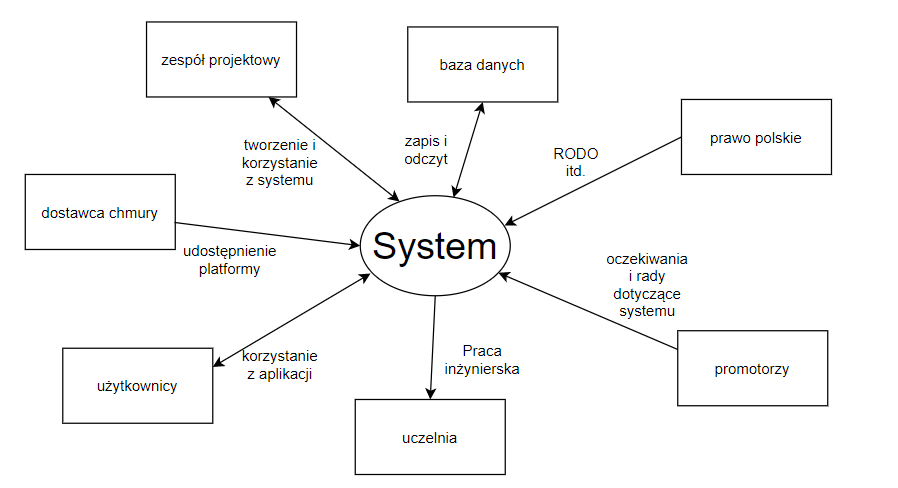
\includegraphics[width=15 cm, left]{system.png}\\
	\item \textbf{Udziałowcy}\\
	\begin{tabular}{|p{3cm}|p{11cm}|}
	\hline
	\multicolumn{2}{|l|}{\textbf{Karta Udziałowca}}\\
	\hline
	Indentyfikator&UOB01\\
	\hline
	Nazwa&Zespół projektowy\\
	\hline
	Opis&Zespół projektowy tworzy oraz opiekuje się systemem\\
	\hline
	Typ udziałowca&Ożywiony, bezpośredni\\
	\hline
	Punkt widzenia&Perspektywa twórców systemu\\
	\hline
	Ograniczenia&Brak\\
	\hline
	Wymagania&\\
	\hline
	\end{tabular}\\
	\begin{tabular}{|p{3cm}|p{11cm}|}
	\hline
	\multicolumn{2}{|l|}{\textbf{Karta Udziałowca}}\\
	\hline
	Indentyfikator&UOB02\\
	\hline
	Nazwa&Użytkownik końcowy\\
	\hline
	Opis&Przeciętny, finalny użytkownik korzystający z aplikacji\\
	\hline
	Typ udziałowca&Ożywiony, bezpośredni\\
	\hline
	Punkt widzenia&Perspektywa użytkownika\\
	\hline
	Ograniczenia&Nie ma dostępu do warstwy technicznej - bazy danych, kodu itp.\\
	\hline
	Wymagania&\\
	\hline
	\end{tabular}\\
	\begin{tabular}{|p{3cm}|p{11cm}|}
	\hline
	\multicolumn{2}{|l|}{\textbf{Karta Udziałowca}}\\
	\hline
	Indentyfikator&UOB03\\
	\hline
	Nazwa&Sponsorzy\\
	\hline
	Opis&Osoba, która finansuje projekt i egzekwuje wymagania\\
	\hline
	Typ udziałowca&Ożywiony, bezpośredni\\
	\hline
	Punkt widzenia&Perspektywa ekonomiczna\\
	\hline
	Ograniczenia&Nie powinien narzucać technologii przy tworzeniu projektu\\
	\hline
	Wymagania&\\
	\hline
	\end{tabular}\\
	\begin{tabular}{|p{3cm}|p{11cm}|}
	\hline
	\multicolumn{2}{|l|}{\textbf{Karta Udziałowca}}\\
	\hline
	Indentyfikator&UOB04\\
	\hline
	Nazwa&Wydawca\\
	\hline
	Opis&Osoba, która jest odpowiedzialna za sfinalizowanie projektu i wypuszczenie go na rynek\\
	\hline
	Typ udziałowca&Ożywiony, bezpośredni\\
	\hline
	Punkt widzenia&Perspektywa ekonomiczna\\
	\hline
	Ograniczenia&Nie powinien narzucać technologii przy tworzeniu projektu\\
	\hline
	Wymagania&\\
	\hline
	\end{tabular}\\
	\begin{tabular}{|p{3cm}|p{11cm}|}
	\hline
	\multicolumn{2}{|l|}{\textbf{Karta Udziałowca}}\\
	\hline
	Indentyfikator&UOB05\\
	\hline
	Nazwa&Promotorzy\\
	\hline
	Opis&Doradcy w sprawach dotyczących projektu\\
	\hline
	Typ udziałowca&Ożywiony, bezpośredni\\
	\hline
	Punkt widzenia&Perspektywa twórców projektu\\
	\hline
	Ograniczenia&Nie zawsze dostępni\\
	\hline
	Wymagania&\\
	\hline
	\end{tabular}\\
	\begin{tabular}{|p{3cm}|p{11cm}|}
	\hline
	\multicolumn{2}{|l|}{\textbf{Karta Udziałowca}}\\
	\hline
	Indentyfikator&UNB01\\
	\hline
	Nazwa&Media\\
	\hline
	Opis&Strony internetowe, reklamy, artykuły, audycje itp.\\
	\hline
	Typ udziałowca&Nieożywiony, bezpośredni\\
	\hline
	Punkt widzenia&Perspektywa ekonomiczna\\
	\hline
	Ograniczenia&Zero wpływu na budowę projektu\\
	\hline
	Wymagania&\\
	\hline
	\end{tabular}\\
	\begin{tabular}{|p{3cm}|p{11cm}|}
	\hline
	\multicolumn{2}{|l|}{\textbf{Karta Udziałowca}}\\
	\hline
	Indentyfikator&UNB02\\
	\hline
	Nazwa&Baza danych\\
	\hline
	Opis&Jedna, wspólna baza danych na cały system\\
	\hline
	Typ udziałowca&Nieożywiony, bezpośredni\\
	\hline
	Punkt widzenia&Perspektywa techniczna\\
	\hline
	Ograniczenia&Skończona ilość pamięci do przechowywanie informacji\\
	\hline
	Wymagania&\\
	\hline
	\end{tabular}\\
	\begin{tabular}{|p{3cm}|p{11cm}|}
	\hline
	\multicolumn{2}{|l|}{\textbf{Karta Udziałowca}}\\
	\hline
	Indentyfikator&UNB03\\
	\hline
	Nazwa&Prawo polskie\\
	\hline
	Opis&Zgodnie z RODO mamy obowiązek dbać o bezpieczeństwo danych osobowych wszyskich użytkowników\\
	\hline
	Typ udziałowca&Nieożywiony, bezpośredni\\
	\hline
	Punkt widzenia&Perspektywa prawna\\
	\hline
	Ograniczenia&Brak\\
	\hline
	Wymagania&\\
	\hline
	\end{tabular}\\
	\begin{tabular}{|p{3cm}|p{11cm}|}
	\hline
	\multicolumn{2}{|l|}{\textbf{Karta Udziałowca}}\\
	\hline
	Indentyfikator&UNB04\\
	\hline
	Nazwa&Dostawca usług chmurowych\\
	\hline
	Opis&Serwer w chmurze odpowiedzialny za przetwarzanie wszystkich żądań pomiędzy serwisami i użytkownikami końcowymi\\
	\hline
	Typ udziałowca&Nieożywiony, bezpośredni\\
	\hline
	Punkt widzenia&Perspektywa techniczna\\
	\hline
	Ograniczenia&Ograniczenia sprzętowe, specyfikacja sprzętu (np. moc procesora serwerowego, przepustowość Internetu)\\
	\hline
	Wymagania&\\
	\hline
	\end{tabular}\\
	\item \textbf{Klienci}\\
	Klienci wewnętrzni:
	\begin{itemize}
		\item Zespół projektowy - grupa odpowiedzialna za wytwarzanie systemu
		\item Wydawca - Product owner, wskazuje wymagania systemu
		\item Sponsorzy - Osoby finansujące projekt
		\item Promotorzy - Osoby nadzorujące  prace nad projektem
	\end{itemize}
	Klienci zewnętrzni:
	\begin{itemize}
		\item Media (redaktorzy, recenzenci itp.) - Strony reklamujące nasz produkt
		\item Użytkownicy końcowi - osoby korzystające z gotowego produktu
	\end{itemize}
	\item \textbf{Role użytkowników systemu}
	\begin{itemize}
		\item gość - dostęp do zakładki ze stroną główną, założeniem konta oraz zalogowaniem się.
		\item Użytkownik zarejestrowany - dostęp do swojego profilu, możliwość korzystania ze wszystkich funkcji jakie oferuje produkt
	\end{itemize}
\end{itemize}
\section{Wymagania}
\begin{itemize}
	\item Wymagania ogólne i dziedzinowe\\
		\begin{tabular}{|p{3cm}|p{2cm}|p{2cm}|p{6cm}|}
		\hline
		\multicolumn{4}{|p{12 cm}|}{Karta Wymagania}\\
		\hline
		Indentyfikator: & W01 & Priorytet: & M - must(musi być)\\
		\hline
		Nazwa & \multicolumn{3}{|p{10 cm}|}{Zwiększenie efektywności pracy użytkowników systemu}\\
		\hline
		Opis & \multicolumn{3}{|p{10 cm}|}{Końcowy produkt systemu ma za zadanie zwiększać produktywność jego użytkowników, weryfikowane jest to na podstawie prac z Harvardu i user feedback’u w postaci ankiet. }\\
		\hline
		Udziałowiec & \multicolumn{3}{|p{10 cm}|}{Wydawca, Użytkownik końcowy}\\
		\hline
		Wymagania powiązane & \multicolumn{3}{|p{10 cm}|}{Brak}\\
		\hline
		\end{tabular}\\
		\begin{tabular}{|p{3cm}|p{2cm}|p{2cm}|p{6cm}|}
		\hline
		\multicolumn{4}{|p{12 cm}|}{Karta Wymagania}\\
		\hline
		Indentyfikator: & W01 & Priorytet: & M - must(musi być)\\
		\hline
		Nazwa & \multicolumn{3}{|p{10 cm}|}{System skórek}\\
		\hline
		Opis & \multicolumn{3}{|p{10 cm}|}{Produkt będzie zarabiał na sprzedaży skórek(alternatywna oprawa graficzna i personalizacja systemu pracy)}\\
		\hline
		Udziałowiec & \multicolumn{3}{|p{10 cm}|}{Wydawca, Sponsorzy}\\
		\hline
		Wymagania powiązane & \multicolumn{3}{|p{10 cm}|}{Brak}\\
		\hline
		\end{tabular}\\
	\item Wymagania funkcjonalne
	\begin{itemize}
		\item Nazwa funkcji/usługi\\
		\begin{tabular}{|p{3cm}|p{2cm}|p{2cm}|p{6cm}|}
		\hline
		\multicolumn{4}{|p{12 cm}|}{Karta Wymagania}\\
		\hline
		Indentyfikator: & F01 & Priorytet: & M - must(musi być)\\
		\hline
		Nazwa & \multicolumn{3}{|p{10 cm}|}{System Autoryzacji użytkownika}\\
		\hline
		Opis & \multicolumn{3}{|p{10 cm}|}{Jako użytkownik muszę mieć możliwość zarejestrowania się w serwisie i późniejszego logowania się}\\
		\hline
		Kryteria akceptacji & \multicolumn{3}{|p{10 cm}|}{Bezpieczny system autoryzacji zabezpieczony przed atakami na baze danych, potwierdzenie maila po rejestracji,  jedno konta na 1 mail}\\
		\hline
		Dane wejściowe & \multicolumn{3}{|p{10 cm}|}{Brak}\\
		\hline
		Warunki początkowe & \multicolumn{3}{|p{10 cm}|}{Brak}\\
		\hline
		Warunki końcowe & \multicolumn{3}{|p{10 cm}|}{Brak}\\
		\hline
		Sytuacje wyjątkowe & \multicolumn{3}{|p{10 cm}|}{Brak}\\
		\hline
		Szczegóły implementacji & \multicolumn{3}{|p{10 cm}|}{Brak}\\
		\hline
		Udziałowiec & \multicolumn{3}{|p{10 cm}|}{Użytkownik końcowy, Zespół projektowy}\\
		\hline
		Wymagania powiązane & \multicolumn{3}{|p{10 cm}|}{Brak}\\
		\hline
		\end{tabular}\\
		\begin{tabular}{|p{3cm}|p{2cm}|p{2cm}|p{6cm}|}
		\hline
		\multicolumn{4}{|p{12 cm}|}{Karta Wymagania}\\
		\hline
		Indentyfikator: & F02 & Priorytet: & M - must(musi być)\\
		\hline
		Nazwa & \multicolumn{3}{|p{10 cm}|}{System rang użytkowników}\\
		\hline
		Opis & \multicolumn{3}{|p{10 cm}|}{Jako użytkownik podczas progresowania w trakcie używania aplikacji chciałbym być przypisywany do różnych rang}\\
		\hline
		Kryteria akceptacji & \multicolumn{3}{|p{10 cm}|}{Przypisywanie rangi do danego użytkownika oraz obliczanie jego statystyk na podstawie wykonywanych projektów}\\
		\hline
		Dane wejściowe & \multicolumn{3}{|p{10 cm}|}{Brak}\\
		\hline
		Warunki początkowe & \multicolumn{3}{|p{10 cm}|}{Brak}\\
		\hline
		Warunki końcowe & \multicolumn{3}{|p{10 cm}|}{Brak}\\
		\hline
		Sytuacje wyjątkowe & \multicolumn{3}{|p{10 cm}|}{Brak}\\
		\hline
		Szczegóły implementacji & \multicolumn{3}{|p{10 cm}|}{Brak}\\
		\hline
		Udziałowiec & \multicolumn{3}{|p{10 cm}|}{Użytkownik końcowy, Zespół projektowy}\\
		\hline
		Wymagania powiązane & \multicolumn{3}{|p{10 cm}|}{Brak}\\
		\hline
		\end{tabular}\\
		\begin{tabular}{|p{3cm}|p{2cm}|p{2cm}|p{6cm}|}
		\hline
		\multicolumn{4}{|p{12 cm}|}{Karta Wymagania}\\
		\hline
		Indentyfikator: & F03 & Priorytet: & M - must(musi być)\\
		\hline
		Nazwa & \multicolumn{3}{|p{10 cm}|}{System zarządzania energią  użytkownika}\\
		\hline
		Opis & \multicolumn{3}{|p{10 cm}|}{Jako użytkownik chcę żeby aplikacja śledziła moje zasoby energetyczne i podpowiadała jak mogę nimi lepiej zarządzać}\\
		\hline
		Kryteria akceptacji & \multicolumn{3}{|p{10 cm}|}{Zmiana zasobów energii użytkownika przy wykonywaniu konkretnych projektów lub przerw}\\
		\hline
		Dane wejściowe & \multicolumn{3}{|p{10 cm}|}{Brak}\\
		\hline
		Warunki początkowe & \multicolumn{3}{|p{10 cm}|}{Brak}\\
		\hline
		Warunki końcowe & \multicolumn{3}{|p{10 cm}|}{Brak}\\
		\hline
		Sytuacje wyjątkowe & \multicolumn{3}{|p{10 cm}|}{Brak}\\
		\hline
		Szczegóły implementacji & \multicolumn{3}{|p{10 cm}|}{Brak}\\
		\hline
		Udziałowiec & \multicolumn{3}{|p{10 cm}|}{Użytkownik końcowy, Zespół projektowy}\\
		\hline
		Wymagania powiązane & \multicolumn{3}{|p{10 cm}|}{Brak}\\
		\hline
		\end{tabular}\\
		\begin{tabular}{|p{3cm}|p{2cm}|p{2cm}|p{6cm}|}
		\hline
		\multicolumn{4}{|p{12 cm}|}{Karta Wymagania}\\
		\hline
		Indentyfikator: & F04 & Priorytet: & M - must(musi być)\\
		\hline
		Nazwa & \multicolumn{3}{|p{10 cm}|}{System zarządzania projektami użytkowników}\\
		\hline
		Opis & \multicolumn{3}{|p{10 cm}|}{Jako użytkownik chciałbym mieć możliwość dodawania, usuwania i śledzenia projektów lub zadań}\\
		\hline
		Kryteria akceptacji & \multicolumn{3}{|p{10 cm}|}{Użytkownik ma możliwość dodawania, usuwania i śledzenia projektów przez siebie stworzonych}\\
		\hline
		Dane wejściowe & \multicolumn{3}{|p{10 cm}|}{Brak}\\
		\hline
		Warunki początkowe & \multicolumn{3}{|p{10 cm}|}{Brak}\\
		\hline
		Warunki końcowe & \multicolumn{3}{|p{10 cm}|}{Brak}\\
		\hline
		Sytuacje wyjątkowe & \multicolumn{3}{|p{10 cm}|}{Brak}\\
		\hline
		Szczegóły implementacji & \multicolumn{3}{|p{10 cm}|}{Brak}\\
		\hline
		Udziałowiec & \multicolumn{3}{|p{10 cm}|}{Użytkownik końcowy, Zespół projektowy}\\
		\hline
		Wymagania powiązane & \multicolumn{3}{|p{10 cm}|}{Brak}\\
		\hline
		\end{tabular}\\
		\begin{tabular}{|p{3cm}|p{2cm}|p{2cm}|p{6cm}|}
		\hline
		\multicolumn{4}{|p{12 cm}|}{Karta Wymagania}\\
		\hline
		Indentyfikator: & F05 & Priorytet: & M - must(musi być)\\
		\hline
		Nazwa & \multicolumn{3}{|p{10 cm}|}{Bullet Journal}\\
		\hline
		Opis & \multicolumn{3}{|p{10 cm}|}{Jako użytkownik chcę mieć możliwość rozplanowania zadań na dni oraz zobaczenia ich rozłożonych w czasie na tablicy lub w postaci kalendarza}\\
		\hline
		Kryteria akceptacji & \multicolumn{3}{|p{10 cm}|}{Użytkownik może dodawać swoje zadania wraz z datami ich wykonania, które zostają zwizualizowane w postaci tablicy lub kalendarza}\\
		\hline
		Dane wejściowe & \multicolumn{3}{|p{10 cm}|}{Brak}\\
		\hline
		Warunki początkowe & \multicolumn{3}{|p{10 cm}|}{Brak}\\
		\hline
		Warunki końcowe & \multicolumn{3}{|p{10 cm}|}{Brak}\\
		\hline
		Sytuacje wyjątkowe & \multicolumn{3}{|p{10 cm}|}{Brak}\\
		\hline
		Szczegóły implementacji & \multicolumn{3}{|p{10 cm}|}{Brak}\\
		\hline
		Udziałowiec & \multicolumn{3}{|p{10 cm}|}{Użytkownik końcowy, Zespół projektowy}\\
		\hline
		Wymagania powiązane & \multicolumn{3}{|p{10 cm}|}{Brak}\\
		\hline
		\end{tabular}\\
		\begin{tabular}{|p{3cm}|p{2cm}|p{2cm}|p{6cm}|}
		\hline
		\multicolumn{4}{|p{12 cm}|}{Karta Wymagania}\\
		\hline
		Indentyfikator: & F06 & Priorytet: & C – could \\
		\hline
		Nazwa & \multicolumn{3}{|p{10 cm}|}{System osiągnięć użytkownika}\\
		\hline
		Opis & \multicolumn{3}{|p{10 cm}|}{Jako użytkownik chciałbym co jakiś czas być nagradzany za osiągnięcia przy dochodzeniu do kamieni milowych podczas korzystania z aplikacji}\\
		\hline
		Kryteria akceptacji & \multicolumn{3}{|p{10 cm}|}{Użytkownik otrzymuje osiągnięcia za przekroczenie pewnych kamieni milowych}\\
		\hline
		Dane wejściowe & \multicolumn{3}{|p{10 cm}|}{Brak}\\
		\hline
		Warunki początkowe & \multicolumn{3}{|p{10 cm}|}{Brak}\\
		\hline
		Warunki końcowe & \multicolumn{3}{|p{10 cm}|}{Brak}\\
		\hline
		Sytuacje wyjątkowe & \multicolumn{3}{|p{10 cm}|}{Brak}\\
		\hline
		Szczegóły implementacji & \multicolumn{3}{|p{10 cm}|}{Brak}\\
		\hline
		Udziałowiec & \multicolumn{3}{|p{10 cm}|}{Użytkownik końcowy, Zespół projektowy}\\
		\hline
		Wymagania powiązane & \multicolumn{3}{|p{10 cm}|}{Brak}\\
		\hline
		\end{tabular}\\
		\begin{tabular}{|p{3cm}|p{2cm}|p{2cm}|p{6cm}|}
		\hline
		\multicolumn{4}{|p{12 cm}|}{Karta Wymagania}\\
		\hline
		Indentyfikator: & F07 & Priorytet: & C – could\\
		\hline
		Nazwa & \multicolumn{3}{|p{10 cm}|}{System rankingowy użytkowników}\\
		\hline
		Opis & \multicolumn{3}{|p{10 cm}|}{Jako użytkownik chciałbym mieć dostęp do tablic rankingowych gdzie mógłbym porównywać swoje osiągniecia z innymi użytkownikami }\\
		\hline
		Kryteria akceptacji & \multicolumn{3}{|p{10 cm}|}{Użytkownik jest w stanie sprawdzić swoją pozycję w rankingu dotyczącą danego projektu}\\
		\hline
		Dane wejściowe & \multicolumn{3}{|p{10 cm}|}{Brak}\\
		\hline
		Warunki początkowe & \multicolumn{3}{|p{10 cm}|}{Brak}\\
		\hline
		Warunki końcowe & \multicolumn{3}{|p{10 cm}|}{Brak}\\
		\hline
		Sytuacje wyjątkowe & \multicolumn{3}{|p{10 cm}|}{Brak}\\
		\hline
		Szczegóły implementacji & \multicolumn{3}{|p{10 cm}|}{Brak}\\
		\hline
		Udziałowiec & \multicolumn{3}{|p{10 cm}|}{Użytkownik końcowy, Zespół projektowy}\\
		\hline
		Wymagania powiązane & \multicolumn{3}{|p{10 cm}|}{Brak}\\
		\hline
		\end{tabular}\\
		\begin{tabular}{|p{3cm}|p{2cm}|p{2cm}|p{6cm}|}
		\hline
		\multicolumn{4}{|p{12 cm}|}{Karta Wymagania}\\
		\hline
		Indentyfikator: & F08 & Priorytet: & C – could \\
		\hline
		Nazwa & \multicolumn{3}{|p{10 cm}|}{System znajomych użytkowników}\\
		\hline
		Opis & \multicolumn{3}{|p{10 cm}|}{Jako użytkownik chciałbym móc dodawać innych użytkowników do swojej listy znajomych żeby sprawdzać ich postępy}\\
		\hline
		Kryteria akceptacji & \multicolumn{3}{|p{10 cm}|}{Użytkownik może dodawaj znajomych, wyświetlanych w formie listy, u których może sprawdzać ich postępy}\\
		\hline
		Dane wejściowe & \multicolumn{3}{|p{10 cm}|}{Brak}\\
		\hline
		Warunki początkowe & \multicolumn{3}{|p{10 cm}|}{Brak}\\
		\hline
		Warunki końcowe & \multicolumn{3}{|p{10 cm}|}{Brak}\\
		\hline
		Sytuacje wyjątkowe & \multicolumn{3}{|p{10 cm}|}{Brak}\\
		\hline
		Szczegóły implementacji & \multicolumn{3}{|p{10 cm}|}{Brak}\\
		\hline
		Udziałowiec & \multicolumn{3}{|p{10 cm}|}{Użytkownik końcowy, Zespół projektowy}\\
		\hline
		Wymagania powiązane & \multicolumn{3}{|p{10 cm}|}{Brak}\\
		\hline
		\end{tabular}\\
		\begin{tabular}{|p{3cm}|p{2cm}|p{2cm}|p{6cm}|}
		\hline
		\multicolumn{4}{|p{12 cm}|}{Karta Wymagania}\\
		\hline
		Indentyfikator: & F09 & Priorytet: & C – could\\
		\hline
		Nazwa & \multicolumn{3}{|p{10 cm}|}{Energy Assistant}\\
		\hline
		Opis & \multicolumn{3}{|p{10 cm}|}{Jako użytkownik chciałbym żeby moje rzeczywiste poziomy energii były lepiej rozpoznawane }\\
		\hline
		Kryteria akceptacji & \multicolumn{3}{|p{10 cm}|}{Użytkownik zależnie jaki prowadzi tryb życia, bądź w zależności od jego warunków fizycznych jak i psychicznych miałby dostosowywaną ilość energii na dany dzień}\\
		\hline
		Dane wejściowe & \multicolumn{3}{|p{10 cm}|}{Brak}\\
		\hline
		Warunki początkowe & \multicolumn{3}{|p{10 cm}|}{Brak}\\
		\hline
		Warunki końcowe & \multicolumn{3}{|p{10 cm}|}{Brak}\\
		\hline
		Sytuacje wyjątkowe & \multicolumn{3}{|p{10 cm}|}{Brak}\\
		\hline
		Szczegóły implementacji & \multicolumn{3}{|p{10 cm}|}{Brak}\\
		\hline
		Udziałowiec & \multicolumn{3}{|p{10 cm}|}{Użytkownik końcowy, Zespół projektowy}\\
		\hline
		Wymagania powiązane & \multicolumn{3}{|p{10 cm}|}{Brak}\\
		\hline
		\end{tabular}\\
		\begin{tabular}{|p{3cm}|p{2cm}|p{2cm}|p{6cm}|}
		\hline
		\multicolumn{4}{|p{12 cm}|}{Karta Wymagania}\\
		\hline
		Indentyfikator: & F10 & Priorytet: & C – could\\
		\hline
		Nazwa & \multicolumn{3}{|p{10 cm}|}{Elastic Habits}\\
		\hline
		Opis & \multicolumn{3}{|p{10 cm}|}{Jako użytkownik chciałbym móc podzielić swoje zadanie na różne poziomy trudności }\\
		\hline
		Kryteria akceptacji & \multicolumn{3}{|p{10 cm}|}{Użytkownik może wybrać z dany poziom trudności zadania by wyrobić sobie nawyk wykonywania go.}\\
		\hline
		Dane wejściowe & \multicolumn{3}{|p{10 cm}|}{Brak}\\
		\hline
		Warunki początkowe & \multicolumn{3}{|p{10 cm}|}{Brak}\\
		\hline
		Warunki końcowe & \multicolumn{3}{|p{10 cm}|}{Brak}\\
		\hline
		Sytuacje wyjątkowe & \multicolumn{3}{|p{10 cm}|}{Brak}\\
		\hline
		Szczegóły implementacji & \multicolumn{3}{|p{10 cm}|}{Brak}\\
		\hline
		Udziałowiec & \multicolumn{3}{|p{10 cm}|}{Użytkownik końcowy, Zespół projektowy}\\
		\hline
		Wymagania powiązane & \multicolumn{3}{|p{10 cm}|}{Brak}\\
		\hline
		\end{tabular}\\
		\item Interfejs z otoczeniem\\
		\begin{tabular}{|p{3cm}|p{2cm}|p{2cm}|p{6cm}|}
		\hline
		\multicolumn{4}{|p{12 cm}|}{Karta Wymagania}\\
		\hline
		Indentyfikator: & I01 & Priorytet: & M – must (musi być)\\
		\hline
		Nazwa & \multicolumn{3}{|p{10 cm}|}{Integracja mikro serwisów}\\
		\hline
		Opis & \multicolumn{3}{|p{10 cm}|}{Nasz projekt strukturalnie będzie zbudowany z wielu mikro serwisów i wymagana jest integracja miedzy nimi(komunikatywność)}\\
		\hline
		Kryteria akceptacji & \multicolumn{3}{|p{10 cm}|}{Funkcje w każdym serwisie umożliwiające komunikowanie się z innymi serwisami}\\
		\hline
		Dane wejściowe & \multicolumn{3}{|p{10 cm}|}{Brak}\\
		\hline
		Warunki początkowe & \multicolumn{3}{|p{10 cm}|}{Brak}\\
		\hline
		Warunki końcowe & \multicolumn{3}{|p{10 cm}|}{Brak}\\
		\hline
		Sytuacje wyjątkowe & \multicolumn{3}{|p{10 cm}|}{Brak}\\
		\hline
		Szczegóły implementacji & \multicolumn{3}{|p{10 cm}|}{Brak}\\
		\hline
		Udziałowiec & \multicolumn{3}{|p{10 cm}|}{Zespół projektowy}\\
		\hline
		Wymagania powiązane & \multicolumn{3}{|p{10 cm}|}{Brak}\\
		\hline
		\end{tabular}\\
		\begin{tabular}{|p{3cm}|p{2cm}|p{2cm}|p{6cm}|}
		\hline
		\multicolumn{4}{|p{12 cm}|}{Karta Wymagania}\\
		\hline
		Indentyfikator: & I02 & Priorytet: & M – must (musi być)\\
		\hline
		Nazwa & \multicolumn{3}{|p{10 cm}|}{Baza danych}\\
		\hline
		Opis & \multicolumn{3}{|p{10 cm}|}{Jedna zintegrowana baza danych dla wszystkich serwisów}\\
		\hline
		Kryteria akceptacji & \multicolumn{3}{|p{10 cm}|}{Baza danych w MongoDB która będzie obsługiwać wszystkie mikro serwisy projektu, będzie posiadała dane użytkowników i wszystkiego co jest związane z aplikacja}\\
		\hline
		Dane wejściowe & \multicolumn{3}{|p{10 cm}|}{Brak}\\
		\hline
		Warunki początkowe & \multicolumn{3}{|p{10 cm}|}{Brak}\\
		\hline
		Warunki końcowe & \multicolumn{3}{|p{10 cm}|}{Brak}\\
		\hline
		Sytuacje wyjątkowe & \multicolumn{3}{|p{10 cm}|}{Brak}\\
		\hline
		Szczegóły implementacji & \multicolumn{3}{|p{10 cm}|}{Brak}\\
		\hline
		Udziałowiec & \multicolumn{3}{|p{10 cm}|}{Zespół projektowy}\\
		\hline
		Wymagania powiązane & \multicolumn{3}{|p{10 cm}|}{Brak}\\
		\hline
		\end{tabular}\\
	\end{itemize}
	\item Wymagania pozafunkcjonalne\\
	\begin{tabular}{|p{3cm}|p{2cm}|p{2cm}|p{6cm}|}
		\hline
		\multicolumn{4}{|p{12 cm}|}{Karta Wymagania}\\
		\hline
		Indentyfikator: & NF01 & Priorytet: & M – must (musi być)\\
		\hline
		Nazwa & \multicolumn{3}{|p{10 cm}|}{C\#}\\
		\hline
		Opis & \multicolumn{3}{|p{10 cm}|}{Serwisy backendowe powinny być napisane w C\#}\\
		\hline
		Udziałowiec & \multicolumn{3}{|p{10 cm}|}{Zespół projektowy, Wydawca}\\
		\hline
		Wymagania powiązane & \multicolumn{3}{|p{10 cm}|}{Brak}\\
		\hline
		\end{tabular}\\
		\begin{tabular}{|p{3cm}|p{2cm}|p{2cm}|p{6cm}|}
		\hline
		\multicolumn{4}{|p{12 cm}|}{Karta Wymagania}\\
		\hline
		Indentyfikator: & NF02 & Priorytet: & M – must (musi być)\\
		\hline
		Nazwa & \multicolumn{3}{|p{10 cm}|}{React.js}\\
		\hline
		Opis & \multicolumn{3}{|p{10 cm}|}{Serwis frontendowy powinien być napisany korzystając z biblioteki React.js}\\
		\hline
		Udziałowiec & \multicolumn{3}{|p{10 cm}|}{Zespół projektowy, Wydawca}\\
		\hline
		Wymagania powiązane & \multicolumn{3}{|p{10 cm}|}{Brak}\\
		\hline
		\end{tabular}\\
		\begin{tabular}{|p{3cm}|p{2cm}|p{2cm}|p{6cm}|}
		\hline
		\multicolumn{4}{|p{12 cm}|}{Karta Wymagania}\\
		\hline
		Indentyfikator: & NF03 & Priorytet: & M – must (musi być)\\
		\hline
		Nazwa & \multicolumn{3}{|p{10 cm}|}{Czas wdrożenia }\\
		\hline
		Opis & \multicolumn{3}{|p{10 cm}|}{System należy wdrożyć do końca semestru zimowego 2020/2021}\\
		\hline
		Udziałowiec & \multicolumn{3}{|p{10 cm}|}{Zespół projektowy, Promotorzy, Uczelnia, Wydawca}\\
		\hline
		Wymagania powiązane & \multicolumn{3}{|p{10 cm}|}{Brak}\\
		\hline
		\end{tabular}\\
		\begin{tabular}{|p{3cm}|p{2cm}|p{2cm}|p{6cm}|}
		\hline
		\multicolumn{4}{|p{12 cm}|}{Karta Wymagania}\\
		\hline
		Indentyfikator: & NF04 & Priorytet: & M – must (musi być)\\
		\hline
		Nazwa & \multicolumn{3}{|p{10 cm}|}{System powinien być dostępny 24 godziny na dobę, 7 dni w tygodniu}\\
		\hline
		Opis & \multicolumn{3}{|p{10 cm}|}{Dostęp do systemu powinien być umożliwiony w dowolnej chwili danego dnia}\\
		\hline
		Udziałowiec & \multicolumn{3}{|p{10 cm}|}{Zespół projektowy, Użytkownik końcowy, Wydawca}\\
		\hline
		Wymagania powiązane & \multicolumn{3}{|p{10 cm}|}{Brak}\\
		\hline
		\end{tabular}\\
	\item Wymagania na środowisko docelowe\\
	\begin{tabular}{|p{3cm}|p{2cm}|p{2cm}|p{6cm}|}
		\hline
		\multicolumn{4}{|p{12 cm}|}{Karta Wymagania}\\
		\hline
		Indentyfikator: & ŚD01 & Priorytet: & M – must (musi być)\\
		\hline
		Nazwa & \multicolumn{3}{|p{10 cm}|}{Kompatybilność przeglądarek}\\
		\hline
		Opis & \multicolumn{3}{|p{10 cm}|}{Produkt końcowy musi być kompatybilny z 3 najnowszymi wersjami popularnych przeglądarek}\\
		\hline
		Kryteria akceptacji & \multicolumn{3}{|p{10 cm}|}{System kompatybilny z 3 najnowszymi wersjami przeglądarek Google Chrome i Mozilla Firefox}\\
		\hline
		Udziałowiec & \multicolumn{3}{|p{10 cm}|}{Zespół projektowy, Użytkownik końcowy, Wydawca}\\
		\hline
		Wymagania powiązane & \multicolumn{3}{|p{10 cm}|}{Brak}\\
		\hline
		\end{tabular}\\
\end{itemize}

\bibliography{bibliography} 
\bibliographystyle{ieeetr}

\end{document}

